\documentclass{article}
\usepackage[utf8]{inputenc}
\usepackage [polish]{babel}
\usepackage[T1]{fontenc}
\usepackage{graphicx}

\title{Project1}
\author{276720 }
\date{December 2022}

\begin{document}

\maketitle

\section{Wprowadzenie teoretyczne}
{\Large Spadek swobodny – ruch odbywający się wyłącznie pod wpływem
 ciężaru (siły grawitacji), bez oporów ośrodka.}
\section{Przebieg eksperymentu}
   \begin{figure}[h!]
  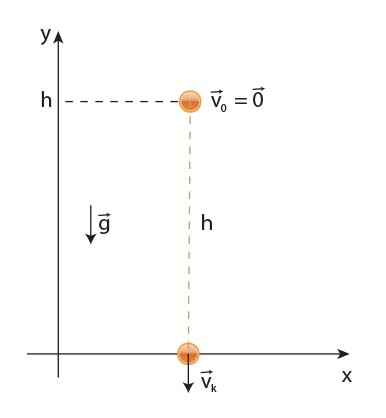
\includegraphics[scale=0.5]{rys0010.jpg}
  \caption{Siły w spadku}
  \label{fig:birds}
\end{figure}

{\Large... Jak widac na rys. \ref{fig:birds}}
\section{Wyniki pomiarów}
\section{Wnioski}

\end{document}
